%\section{Title @Venue'Year}
%\subsection{Background/Problems}
%\subsection{Methods/Techniques}
%\subsection{Results/Evaluation}
%\subsection{Limitations/Comments}
%\newpage
%\begin{figure}[h]
%    \centering
%    \includegraphics[width=\linewidth]{xx.png} %
%    \caption{xx's arch.}	
%    \label{fig:xx}
%\end{figure}
\documentclass[10pt]{article} %twocolumn
%\usepackage{ctex}
\usepackage{titlesec}
\usepackage{titletoc}
\titleformat*{\section}{\normalfont\bfseries} %\tiny\scriptsize\footnotesize\small\normalsize\large\Large\LARGE\huge\Huge
\titleformat*{\subsection}{\normalfont\bfseries}
\usepackage{graphicx}
\usepackage{url}
\usepackage{listings}
\usepackage[colorlinks,linkcolor=black,anchorcolor=blue,citecolor=green]{hyperref}%
%for pdftex
%\setlength{\pdfpageheight}{160mm}
%\setlength{\pdfpagewidth}{80mm}

%for dvipdfm
%\special{pdf: pagesize width 80mm height 160mm}

%\setcounter{secnumdepth}{3}		%编号深度
\setcounter{tocdepth}{1}		%目录深度
\titlecontents{section}[0mm]%标签距离页面左边距
{\footnotesize}
%{\fontsize{10pt}{10pt}} %\selectfont
{\contentslabel{1em}}  %标签距离目录内容距离
{}
{\titlerule*{.}\contentspage}[\addvspace{.5pc}]


\let\phone=1 %-------------生成适合手机上阅读的pdf文件;否则注释此行。------------------
\ifx\phone1
\usepackage[centering,margin=0.5cm]{geometry}
\geometry{papersize={12cm,20cm}} 
\else
\usepackage[a4paper,margin=2cm]{geometry}%,left=2cm,right=2cm,top=1cm,bottom=1cm
\twocolumn
\fi


%for dvips
%\special{papersize=80mm,160mm} %dvi 没有纸张大小的概念,只有转换成 .ps、.pdf 文件时,才由对应的输出驱动(如 Dvips、dvipdfmx 或 pdfTeX 等)设置输出纸张大小。
%传统的 TeX 代码里面本身不能直接设置纸大小,因此才需要在安装 TeX Live 时选择那些输出驱动的默认纸张大小。而 article 等文档类的 a4paper、letterpaper 选项,只是设置合适的版心位置和距离,以适合这些纸张大小。
%不过,在 TeX 代码里面用特定输出驱动的 special 命令,可以提示这些输出驱动选择纸张,一般用 geometry 宏包的话,就会处理这个问题。而 graphics 宏包后台对 pdfTeX 也有相应的代码(在 pdftex.def 中)。


\title{\textbf{Reading Notes}}%文献阅读笔记
\author{\texttt{TSISers} 
    \\ \copyright Trusted Software and Intelligent System Lab.}
\date{2020/01/21}

\begin{document}

\maketitle 
\tableofcontents
\clearpage



\section{SAVIOR: Towards Bug-Driven Hybrid Testing @S\&P'20
}

\subsection{Background/Problems}
Hybrid testing combines fuzzing and concolic execution. It leverages fuzzing to test easy-to-reach code regions and uses concolic execution to explore code blocks guarded by complex branch conditions. As a result, hybrid testing is able to reach deeper into program state space than fuzz testing or concolic execution alone. Recently, hybrid testing has seen significant advancement. However, {its code coverage-centric design is inefficient in vulnerability detection}. First, it {blindly} selects seeds for concolic execution and aims to explore new code continuously. However, as statistics show, a large portion of the explored code is often bug-free. Therefore, giving equal attention to every part of the code during hybrid testing is a non-optimal strategy. It slows down the detection of real vulnerabilities by over 43\%. Second, classic hybrid testing quickly moves on after reaching a chunk of code, rather than examining the hidden defects inside. It may frequently {miss subtle vulnerabilities} despite that it has already explored the vulnerable code paths.
\subsection{Methods/Techniques}
The authors propose SAVIOR (Fig.\ref{fig:savior}), a new hybrid testing framework pioneering a bug-driven principle.

\textbf{Bug-driven prioritization:} Instead of running all seeds without distinction in concolic execution, SAVIOR prioritizes those that have higher possibilities of leading to vulnerabilities.  Specifically, before the testing, SAVIOR analyzes the source code and {statically labels the potentially vulnerable locations} in the target program.  Moreover, SAVIOR computes the set of basic blocks reachable from each branch. During dynamic testing, SAVIOR {prioritizes the concolic execution seeds that can visit more important branches} (i.e., branches whose reachable code has more vulnerability labels).  

\textbf{Bug-guided verification: }Aside from accelerating vulnerability detection, SAVIOR also verifies the labeled vulnerabilities along the program path traversed by the concolic executor.  Specifically, SAVIOR synthesizes the faulty constraint of triggering each vulnerability on the execution path. If such constraint under the current path condition is satisfiable, SAVIOR solves the constraint to construct a test input as the proof. Otherwise, SAVIOR proves that the vulnerability is infeasible on this path, regardless of the input.

\begin{figure}[h]
    \centering
    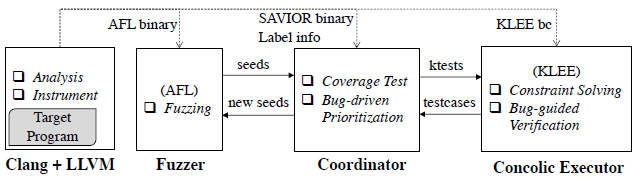
\includegraphics[width=\linewidth]{savior.png} %
    \caption{SAVIOR's arch.}	
    \label{fig:savior}
\end{figure}


\subsection{Results/Evaluation %评估效果
}
Evaluation shows that the bug-driven approach outperforms mainstream hybrid testing systems driven by code coverage. On average, SAVIOR detects vulnerabilities 43.4\% faster than DRILLER and 44.3\% faster than QSYM, leading to the discovery of 88 and 76 more unique bugs, respectively. According to the {evaluation on 11 well fuzzed benchmark programs, within the first 24 hours, SAVIOR triggers 481 UBSAN violations, among which 243 are real bugs.} 
\subsection{Limitations/Comments}
\begin{itemize}
    \item Over-approximation in Vulnerability Labeling: SAVIOR leverages sound algorithms to label vulnerabilities where the over-approximation may introduce many false-positive labels. This imprecision can consequently weaken the performance of SAVIOR's prioritization.  One solution is to include more precise static analysis for finer-grained label pruning.
    \item Prediction in Vulnerability Detection: Once reaching a potentially vulnerable location in concolic execution, SAVIOR extracts the guarding predicates of the vulnerability label. However, these predicates may contradict the current path condition. In case of such contradiction, SAVIOR terminates the exploration of the labeling site immediately.  Moreover, we can predict whether an execution path can trigger a vulnerability or not by studying the runtime information of previous executions, more importantly, before that execution arrives the vulnerability site. To achieve this goal, we need to backwardly summarize path constraints from the labeled site to its predecessors in the explored paths, by using the weakest precondition.
    \item Hybrid testing in SAVIOR is same with hybrid fuzzing in Driller and Berry. Both tools run fuzzing for code exploration and invoke concolic execution only on hard-to-solve branches, which takes advantage of both fuzzer's efficiency and concolic executor's constraint solving.
\end{itemize}
\newpage
\section{Fuzzing File Systems via Two-Dimensional Input Space Exploration @S\&P'19}
\subsection{Background/Problems}
File systems are too big and too complex to be bug free. Nevertheless, to find bugs in file systems, regular stress-testing tools and formal checkers are limited due to the ever-increasing complexity of both file systems and OSes. Thus, fuzzing becomes a preferable choice, as it does not need much knowledge about a target. However, three prominent issues of existing file systems fuzzers exist: (1) fuzzing a large blob image is inefficient; (2) fuzzers do not exploit the dependence between a file system image and file operations; (3) fuzzers use aging OSes and file systems, which results in irreproducible bugs.

\subsection{Methods/Techniques}
The authors present JANUS (Fig.\ref{fig:janus}, 120K C++/C LoC), the first feedback-driven fuzzer that explores the two-dimensional input space of a file system, i.e., mutating metadata on a large image, while emitting image-directed file operations. In addition, JANUS relies on a library OS rather than on traditional VMs for fuzzing, which enables JANUS to load a fresh copy of the OS, thereby leading to better reproducibility of bugs.
\begin{figure}[h]
    \centering
    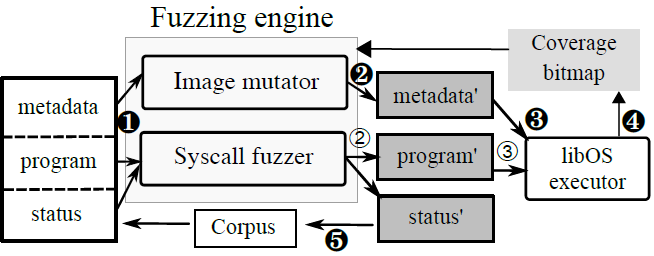
\includegraphics[scale=0.5]{janus.png} %
    \caption{JANUS' arch.}	
    \label{fig:janus}
\end{figure}
\subsection{Results/Evaluation}
The authors evaluate JANUS on 8 file systems and found 90 bugs in the upstream Linux kernel, 62 of which have been acknowledged. 43 bugs have been fixed with 32 CVEs assigned. In addition, JANUS achieves higher code coverage on all the file systems after fuzzing 12 hours, when compared with the state-of-the-art fuzzer Syzkaller.  JANUS visits 4.19X and 2.01X more code paths in Btrfs and ext4, respectively. Moreover, JANUS is able to reproduce 88–100\% of the crashes, while Syzkaller fails on all of them.
\subsection{Limitations/Comments}
\begin{itemize}
    \item JANUS cannot fuzz the DAX mode of a file system without modification on LKL. 
    \item To achieve a minimal PoC, JANUS uses a brute force approach to revert every mutated byte and also tries to remove every invoked file operation to check whether the kernel still crashes at the expected location, which is sub-optimal.
    \item JANUS does not support file systems (e.g., NTFS, GVfs, SSHF, etc.) that rely on FUSE (Filesystem in Userspace).
    \item By combining Janus and kAFL, we can fuzz file systems on other OSes.
    \item Other crash-consistency checkers [6,73] and semantic correctness checkers [36, 58] can rely on or integrate with Janus which aims to find general security bugs in file systems.
    \item To find security bugs in OSes, a number of general kernel fuzzing frameworks [20, 43, 46, 61] and OS-specific kernel fuzzers [22, 25, 44, 45, 47] have been proposed. Unlike JANUS, all these fuzzers generate random system calls based upon predefined grammar rules, which is ineffective in the context of file system fuzzing. Several recent OS fuzzers such as IMF [22] and MoonShine [49] focusing on seed distillation are orthogonal to this work. Nevertheless, JANUS can start with seed programs of high quality by utilizing their approaches.
\end{itemize}
\newpage

\section{REDQUEEN: Fuzzing with Input-to-State Correspondence @NDSS'19}
\subsection{Background/Problems}
Two common problems of fuzzing are magic numbers and (nested) checksums (see Listing \ref{fuzzissues}). Computationally expensive methods such as taint tracking and symbolic execution are typically used to overcome such roadblocks. Unfortunately, such methods often require access to source code, a rather precise description of the environment (e.g., behavior of library calls or the underlying OS), or the exact semantics of the platform's instruction set, and thus such methods are the polar opposite of the approach pioneered by AFL: to a large extend, AFL's success is based on the fact that it makes few assumptions about the program's behavior.
\begin{lstlisting}[label=fuzzissues,language={[ANSI]C}, caption={Roadblocks for feedback-driven fuzzing.}]
/* magic number example */
if(u64(input)==u64("MAGICHDR"))
  bug(1);
/* nested checksum example */
if(u64(input)==sum(input+8, len-8))
  if(u64(input+8)==sum(input+16, len-16))
    if(input[16]=='R' && input[17]=='Q')
      bug(2);
\end{lstlisting}

\subsection{Methods/Techniques}
The authors introduce a lightweight, yet very effective approach to facilitate and optimize state-of-the-art feedback fuzzing that easily scales to large binary applications and unknown environments. They observe that during the execution of a given program, parts of the input often end up directly (i.e., nearly unmodified) in the program state. This \emph{input-to-state correspondence} can be exploited to create a robust method to overcome common fuzzing roadblocks in a highly effective and efficient manner.  Their prototype implementation, called REDQUEEN, is able to solve magic bytes and (nested) checksum tests automatically for a given binary executable. Additionally, The authors show that the techniques outperform various state-of-the-art tools on a wide variety of targets across different privilege levels (kernel-space and userland) with no platform-specific code.
\subsection{Results/Evaluation}
REDQUEEN is the first method to find more than 100\% of the bugs planted in LAVA-M across all targets. Furthermore, The authors discovered 65 new bugs and obtained 16 CVEs in multiple programs and OS kernel drivers. Finally, their evaluation demonstrates that REDQUEEN is fast, widely applicable and outperforms concurrent approaches by up to three orders of magnitude. Available at: \url{https://github.com/RUB-SysSec/redqueen}
\subsection{Limitations/Comments}
\begin{itemize}
    \item REDQUEEN cannot deal with those cases in which the input does not correspond to the state, such as compression or hash maps in the input.
    \item It would be beneficial to use this lightweight approach as a first step where possible, and than solve the remaining challenges using complex approaches.
\end{itemize}

\subsection*{Core design of AFL}
\hspace{2mm}{
Fuzzers from the AFL family have three important components: (i) the queue, (ii) the bitmap, and (iii) the mutators. The queue is where all inputs are stored. During the fuzzing process, an input is picked from the queue, fuzzed for a while, and, eventually, returned to the queue. After picking one input, the mutators perform a series of mutations. After each step, the mutated input is executed. The target is instrumented such that the coverage produced by the input is written into a bitmap. If the input triggered new coverage (and, therefore, a new bit is set in the bitmap), the input is appended to the queue.  Otherwise, the mutated input is discarded. The mutators are organized in different stages. The first stages are called the \emph{deterministic stages}. These stages are applied once, no matter how often the input is picked from the queue. They consist of a variety of simple mutations such as “try flipping each bit”. When the deterministic stages are finished or an input is picked for the second time, the so called \emph{havoc phase} is executed. During this phase, multiple random mutations are applied at the same time at random locations. Similarly, if the user provided a dictionary with interesting strings, they are added in random positions. Linked to the havoc stage is the \emph{splicing stage}, in which two different inputs are combined at a random position.}
\newpage

\section{Grimoire: Synthesizing Structure while Fuzzing @Security'19 }
\subsection{Background/Problems}
One common challenge for current fuzzing techniques are programs which process highly structured input languages such as interpreters, compilers, text-based network protocols or markup languages. Typically, such inputs are consumed by the program in two stages: parsing and semantic analysis. If parsing of the input fails, deeper parts of the target program—containing the actual application logic—fail to execute; hence, bugs hidden “deep” in the code cannot be reached. Even advanced feedback fuzzers— such as AFL—are typically unable to produce diverse sets of syntactically valid inputs.

Previous approaches to address this problem are typically based on manually provided grammars or seed corpora. On the downside, such methods require human experts to (often manually) specify the grammar or suitable seed corpora, which becomes next to impossible for applications with undocumented or proprietary input specifications. An orthogonal line of work tries to utilize advanced program analysis techniques to automatically infer grammars. Typically performed as a pre-processing step, such methods are used for generating a grammar that guides the fuzzing process. However, since this grammar is treated as immutable, no additional learning takes place during the actual fuzzing run.

\subsection{Methods/Techniques}
The authors present the design and implementation of Grimoire (Fig.\ref{fig:grimoire}), a fully automated coverage-guided fuzzer which works without any form of human interaction or pre-configuration; yet, it is still able to efficiently test programs that expect highly structured inputs. Thet achieve this by performing large-scale mutations in the program input space using grammar-like combinations to synthesize new highly structured inputs without any pre-processing step. 

 Their approach is based on two key observations: First, they can use code coverage feedback to automatically infer structural properties of the input language. Second, the precise and “correct” grammars generated by previous approaches are actually unnecessary in practice: since fuzzers have the virtue of high test case throughput, they can deal with a significant amount of noise and imprecision. In fact, in some programs (such as Boolector) with a rather diverse set of input languages, the additional noise even benefits the fuzz testing. In a similar vein, there are often program paths which can only be accessed by inputs outside of the formal specifications, e. g., due to incomplete or imprecise implementations or error handling code.
\begin{figure}[h]
    \centering
    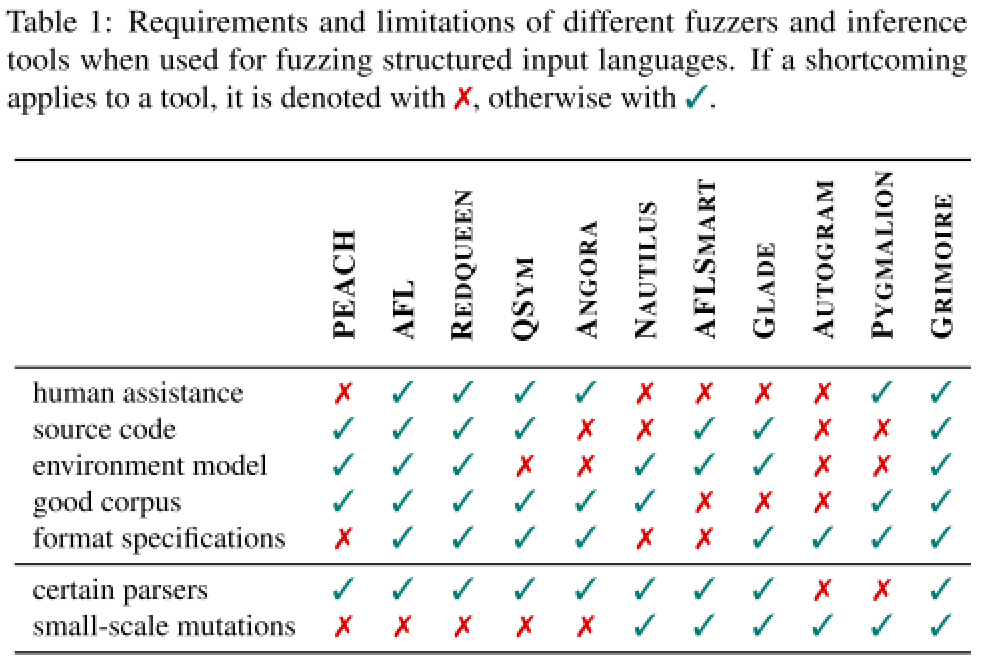
\includegraphics[width=0.6\linewidth]{grimoire.png} %
    \caption{Advantage of Grimoire.}	
    \label{fig:grimoire}
\end{figure}
\subsection{Results/Evaluation}
 First, The authors evaluate Grimoire against other fuzzers on four scripting language interpreters (mruby, PHP, Lua and JavaScriptCore), a compiler (TCC), an assembler (NASM), a database (SQLite), a parser (libxml) and an SMT solver (Boolector).  Grimoire outperforms all existing coverage-guided fuzzers; in the case of Boolector, Grimoire finds up to 87\% more coverage than the baseline (REDQUEEN). 

 Second, they evaluate Grimoire against state-of-the-art grammar-based fuzzers. they observe that in situations where an input specification is available, it is advisable to use Grimoire in addition to a grammar fuzzer to further increase the test coverage found by grammar fuzzers.
 
 Third, they evaluate Grimoire against current state-of-the-art approaches that use automatically inferred grammars for fuzzing and found that they can significantly outperform such approaches. Overall, Grimoire found 19 distinct memory corruption bugs that they manually verified. they responsibly disclosed all of them to the vendors and obtained 11 CVEs. During their evaluation, the next best fuzzer only found 5 of these bugs. In fact, Grimoire found more bugs than all five other fuzzers combined. Available at: \url{https://github.com/RUB-SysSec/grimoire}
\subsection{Limitations/Comments}
The approach has significant difficulties with more syntactically complex constructs, such as matching the ID of opening and closing tags in XML or identifying variable constructs in scripting languages. 

The generalization approach might be too coarse in many places. Obtaining more precise rules would help uncovering deeper parts of the target application in cases where multiple valid statements have to be produced. 
\newpage
\section{Intriguer: Field-Level Constraint Solving for Hybrid Fuzzing @CCS'19}
\subsection{Background/Problems}
Hybrid fuzzing is promising in light of the recent performance improvements in concolic engines. However, there is room for further improvement: symbolic emulation is still slow, unnecessary constraints dominate solving time, resources are overly allocated, and hard-to-trigger bugs are missed.

\subsection{Methods/Techniques}
The authors present a new hybrid fuzzer named Intriguer (Fig.\ref{fig:intriguer}). The key idea of Intriguer is field-level constraint solving, which optimizes symbolic execution with field-level knowledge. Intriguer performs instruction-level taint analysis and records execution traces without data transfer instructions like mov. Intriguer then reduces the execution traces for tainted instructions that accessed a wide range of input bytes, and infers input fields to build field transition trees. With these optimizations, Intriguer can efficiently perform symbolic emulation for more relevant instructions and invoke a solver for complicated constraints only.

\begin{figure}[h]
    \centering
    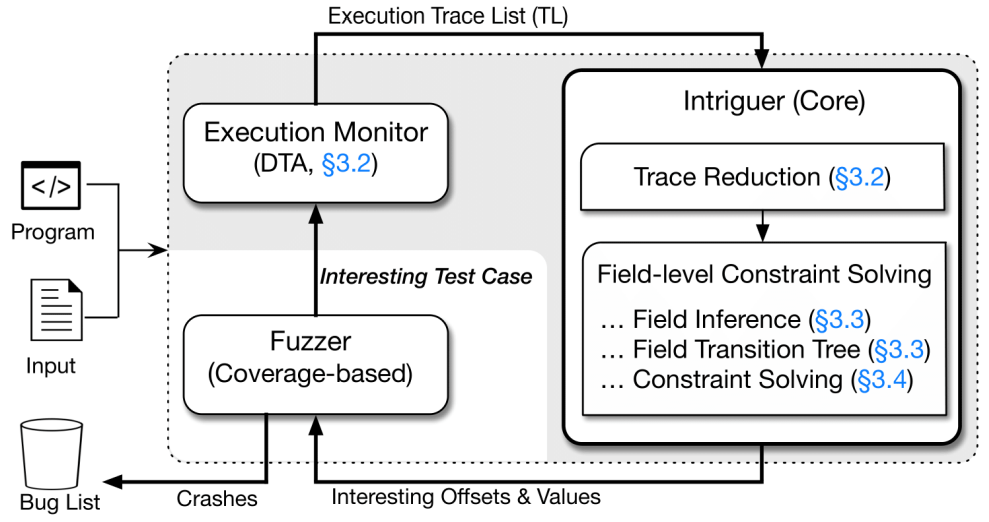
\includegraphics[width=\linewidth]{intriguer.png} %
    \caption{Intriguer's arch.}	
    \label{fig:intriguer}
\end{figure}
\subsection{Results/Evaluation}
Evaluation results indicate that Intriguer outperforms the state-of-the-art fuzzers: Intriguer found all the bugs in the LAVA-M(5h) benchmark dataset for ground truth performance, and also discovered 43 new security bugs in seven real-world programs. They reported the bugs and received 23 new CVEs.

\subsection{Limitations/Comments}
 Intriguer performed field inference by inspecting off sets recorded in the execution traces and did not consider the association between those fields.  To perform field-level constraint solving more efficiently, Intriguer should identify fields of the same type through the FL and grouping them together. In addition to identifying repeated fields, we may infer structure from those fields and then consider mutation strategies specific to repeated fields based on it.

Intriguer reduces the execution traces to emulate only the small portion of the instructions that are repeatedly used to access a wide range of input bytes. One may have two concerns regarding trace reduction. First, excessively reduced traces may affect a constraint solving for important branches. By considering the context-sensitivity of the run-time process, Intriguer will not perform trace reduction when a program is in a different context (e.g., different call stack). Second, the instructions can be repeatedly used to access only a narrow range of input bytes. Note that an execution bottleneck can also occur if the instructions are used to repetitively access the input with specific offsets. We can address this problem by reducing the execution traces for the instructions that use the same offset by considering the program’s context.

Intriguer currently supports most of the x86 instruction set and a part of x86\_64 instruction set. Although it is challenging to support all of x86\_64 instructions, we can implement frequently used instructions to support actual program execution.

The current version of Intriguer does not consider the control-flow dependency, e.g., occurring from indirect
and conditional jump.
\newpage

\section{FIRM-AFL: High-Throughput Greybox Fuzzing of IoT Firmware via Augmented Process Emulation @Sec'19}
\subsection{Background/Problems}
Two fundamental problems in \emph{IoT fuzzing} due to its strong dependency on the actual hardware configuration: 1) Compatibility issues by enabling fuzzing for POSIX-compatible firmware that can be emulated in a system emulator. 2) Performance bottleneck caused by system-mode emulation. 
\subsection{Methods/Techniques}
A novel technique called augmented process emulation. By combining system-mode emulation  (high generality and low efficiency)  and user-mode emulation  (low generality and high efficiency) in a novel way, augmented process emulation provides high compatibility as system-mode emulation and high throughput as user-mode emulation.  The program to be fuzzed is mainly run in user-mode emulation to achieve high efficiency, and switches to full system emulation only when necessary to ensure correct program execution. 
\begin{figure}[h]
    \centering
    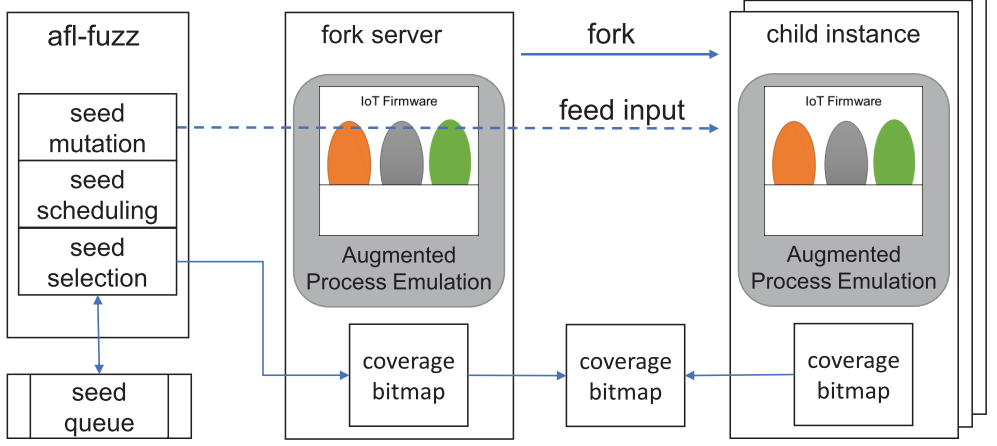
\includegraphics[width=\linewidth]{firm-afl.png} %width=\linewidth
    \caption{firm-afl's arch.}	
    \label{fig:firmafl}
\end{figure}
\subsection{Results/Evaluation}
Evaluation results show that (1) FIRM-AFL is fully functional and capable of finding real-world vulnerabilities in IoT programs; (2) the throughput of FIRM-AFL is on average 8.2 times higher than system-mode emulation based fuzzing; and (3) FIRM-AFL can find 1-day vulnerabilities much faster than system-mode emulation based fuzzing, and find 0-day vulnerabilities.

available at \url{https://github.com/zyw-200/FirmAFL}.

\subsection{Limitations/Comments}
FIRM-AFL only supports the following CPU architectures: mipsel, mipseb and armel.  It can also only fuzz a program in a firmware image that can be properly emulated by Firmadyne and runs a POSIX-compatible OS (e.g., Linux).
\clearpage

\section{RVFUZZER: Finding Input Validation Bugs in Robotic Vehicles Through
Control-Guided Testing @Security'19}
\subsection{Background/Problems}
Attack surface of robotic vehicles (RVs) spans multiple aspects, such as (1) physical vulnerabilities of its sensors that enable external sensor spoofing attacks [72,77,80]; (2) traditional “syntactic” bugs in its control program (e.g., memory corruption bugs) that enable remote or trojaned exploits [75]; and (3) control-semantic bugs in its control program that enable attacks via remote control commands.  For attacks exploiting (1) and (2), there have been research efforts in defending against them [30,38,40,50,52,70,76]; whereas those exploiting (3) have not received sufficient attention. 

 In this paper, the authors address a new type of vulnerability in RV control programs, called input validation bugs, which involve missing or incorrect validation checks on control parameter inputs. Such bugs can be exploited to cause physical disruptions to RVs which may result in mission failures and vehicle damages or crashes. Furthermore, attacks exploiting such bugs have a very small footprint: just one innocent-looking ground control command, requiring no code injection, control flow hijacking or sensor spoofing. 
\subsection{Methods/Techniques}
Testing RV control programs to find input validation bugs is challenging due to many different RV models (e.g., quadcopters and ground rovers) with a large number of hardware, software and control configuration options. Moreover, traditional fuzzing techniques are not directly applicable to RV control programs because: (1) With hundreds of configurable parameters, the control program has an extremely large input space to explore and (2) there is no uniform and obvious condition to automatically decide that a control program is malfunctioning. Many input validation bugs do not exhibit system-level symptoms until certain control and physical conditions are met at run-time.

Our solution to finding input validation bugs – without control program source code – is motivated by the following ideas: (1) The impacts of attacks exploiting input validation bugs can be manifested by the victim vehicle’s control state; and (2) such state can be efficiently reproduced by combining the RV control program and a high-fidelity RV simulation framework, which is readily available [7,8].

Based on these ideas, they develop RVFUZZER (Fig.\ref{fig:rvfuzzer}), a vetting system for finding input validation bugs in RV control programs through control-guided input mutation. The key insight behind RVFUZZER is that the RV control model, which is the generic theoretical model for a broad range of RVs, provides helpful semantic guidance to improve bug-discovery accuracy and efficiency. Specifically, RVFUZZER involves a control instability detector that detects control program misbehavior, by observing (simulated) physical operations of the RV based on the control model. In addition, RVFUZZER steers the input generation for finding input validation bugs more efficiently, by leveraging results from the control instability detector as feedback. 
\begin{figure}[h]
    \centering
    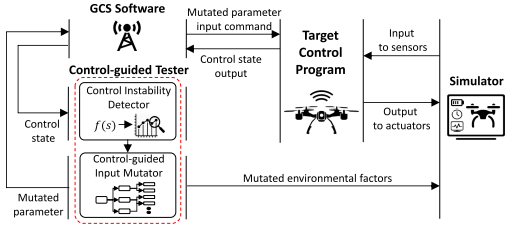
\includegraphics[width=\linewidth]{rvfuzzer.png} %
    \caption{rvfuzzer's arch.}	
    \label{fig:rvfuzzer}
\end{figure}
\subsection{Results/Evaluation}
In their evaluation of RVFUZZER on two popular RV control programs (ArduPilot [15] and PX4 [24]), a total of 89 input validation bugs are found, with 87 of them being zero-day bugs.
\subsection{Limitations/Comments}
The control parameters may have dependencies on one another.  In this work, they consider the subject control program binary as a black box and take a pragmatic approach by only revealing part of such inter-dependencies. A more generic approach to control parameter dependency derivation – possibly based on source code and a formal control model – is left as future work.

There has been no standard safety testing framework created for RVs. We believe that RVFUZZER’s post-production, black-box-based vetting will serve as a useful complement to standardized safety testing during RV design and production.

\newpage
\section{ProFuzzer: On-the-fly Input Type Probing for Better
Zero-day Vulnerability Discovery @S\&P'19}
\subsection{Background/Problems}
Existing mutation based fuzzers tend to randomly mutate the input of a program without understanding its underlying syntax and semantics.  This information (fields and their semantics) may not be documented and available to the fuzzer, and can be hard to recover without going through an in-depth heavyweight analysis procedure. 
\subsection{Methods/Techniques}
 In this paper, the authors propose a novel on-the-fly probing technique (called ProFuzzer, Fig.\ref{fig:profuzzer}) that automatically recovers and understands input fields of critical importance to vulnerability discovery during a fuzzing process and intelligently adapts the mutation strategy to enhance the chance of hitting zero-day targets. Since such probing is transparently piggybacked to the regular fuzzing, no prior knowledge of the input specification is needed. During fuzzing, individual bytes are first mutated and their fuzzing results are automatically analyzed to link those related together and identify the type for the field connecting them; these bytes are further mutated together following type-specific strategies, which substantially prunes the search space.  They define the probe types generally across all applications, thereby making their technique application agnostic.

ProFuzzer is inspired by two important observations. First, a comprehensive, application-specific and semantically rich input specification is not necessary for fuzzing.  Second, inputs can be understood and their fields and data types can be discovered by directly observing the fuzzing process, particularly the ways the input content is mutated and the program’s execution path variations in response to the mutations. 

\begin{figure}[h]
    \centering
    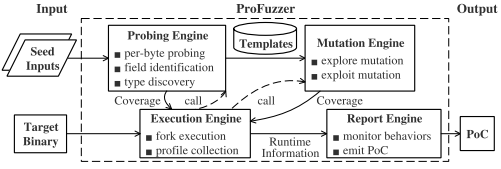
\includegraphics[width=\linewidth]{profuzzer.png} %
    \caption{profuzzer's arch.}	
    \label{fig:profuzzer}
\end{figure}
\subsection{Results/Evaluation}
Eexperiments on standard benchmarks and real-world applications show that ProFuzzer substantially outperforms AFL and its optimized version AFLFast, as well as other state-of-art fuzzers including VUzzer, Driller and QSYM. Within two months, it exposed 42 zero-days in 10 intensively tested programs, generating 30 CVEs.
\subsection{Limitations/Comments}
Currently, the exploitation mutation procedure requires domain knowledge and manual efforts.  A future work is the automatic learning of exploitation rules from a larger pool of PoC.

Review the assumptions that the target application has the following properties. First, its execution is deterministic: that is, given the same input, multiple executions of the application all follow the same execution path and yield the same result. Second, initial valid seed inputs of reasonable size are available. Third, if the validation on certain bytes fails, the execution will quickly terminate, which means that an exceptional execution has a shorter execution path than a normal one. 
\newpage
\section{RetroWrite: Statically Instrumenting COTS Binaries for Fuzzing and Sanitization @S\&P'20}
\subsection{Background/Problems}
The current state of the art for applying fuzzing or sanitization to binaries is dynamic binary translation, which has prohibitive performance overhead. The alternate technique, static binary rewriting, cannot fully recover symbolization information and hence has difficulty modifying binaries to track code coverage for fuzzing or to add security checks for sanitizers.
\subsection{Methods/Techniques}
In this paper, the authors show that static binary rewriting, leveraging reassembleable assembly, can produce sound and efficient code for an important class of binaries: \emph{64-bit position-independent code (PIC)}. Notably, such binaries include third party shared libraries, the analysis of which is the most pressing use-case for such a rewriter. The rewriting technique, called RetroWrite (Fig.\ref{fig:retrowrite}), leverages relocation information which is required for position independent code, and produces assembly files that can be reassembled into binaries. 
\begin{figure}[h]
    \centering
    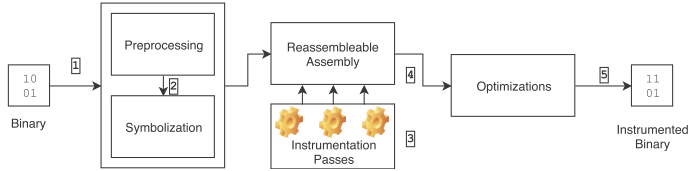
\includegraphics[width=\linewidth]{retrowrite.png} %
    \caption{retrowrite's arch.}	
    \label{fig:retrowrite}
\end{figure}
\subsection{Results/Evaluation}
Binaries rewritten for coverage-guided fuzzing using RetroWrite are identical in performance to compiler-instrumented binaries and outperform the default QEMU-based instrumentation by 4.5x while triggering more bugs. Their implementation of binary-only Address Sanitizer is 3x faster than Valgrind’s memcheck, the state-of-the-art binary-only memory checker, and detects 80\% more bugs in the evaluation.  Available at: \url{https://github.com/HexHive/retrowrite}.
\subsection{Limitations/Comments}
a) Support for C++ Binaries: The current implementation of RetroWrite cannot rewrite C++ binaries safely due to missing symbolization for C++ exception handlers. 

b) Closing the Performance Gap:  Another opportunity to reduce overhead is to remove unnecessary checks when a memory access is known to be safe, e.g., accessing variables on stack through constant offsets from the stack top. 

c) Limitations of ASan-retrowrite: The limitations of ASan-retrowrite on stack and global sections are fundamental to static binary rewriting. To improve precision on stack and data sections, we may need to trade-off soundness or scalability. One attractive option is to use local symbolic execution to track base-pointers and disambiguate references.  

d) Obfuscation: To protect intellectual property, some vendors ship obfuscated binaries. Retrowrite does not address obfuscation. Binary unpacking is usually specific to the obfuscation scheme used; and an obfuscated binary may be rewritten by RetroWrite, after it is pre-processed by a de-obfuscation step [57], [58].
\newpage
\section{SLAKE: Facilitating Slab Manipulation for Exploiting
Vulnerabilities in the Linux Kernel @CCS'19}

\subsection{Background/Problems}
To determine the exploitability for a kernel vulnerability, a security analyst usually has to manipulate slab and thus demonstrate the capability of obtaining the control over a program counter or performing privilege escalation. However, this is a lengthy process because (1) an analyst typically has no clue about what objects and system calls are useful for kernel exploitation and (2) he lacks the knowledge of manipulating a slab and obtaining the desired layout. In the past, researchers have proposed various techniques to facilitate exploit development. Unfortunately, none of them can be easily applied to address these challenges due to the complexity of the Linux kernel and the dynamics and non-deterministic of slab variations.
\subsection{Methods/Techniques}
To tackle the challenges, the authors first use static and dynamic analysis techniques to explore the kernel objects, and the corresponding system calls useful for exploitation. Second, they model commonly-adopted exploitation methods and develop a technical approach to facilitate the slab layout adjustment. By extending LLVM as well as Syzkaller, they implement the techniques and name their combination after SLAKE. 

 More specifically, they first perform reachability analysis over the call graph and preserve only those system calls that could potentially reach to the sites of interest. For each site of interest, they then perform fuzz testing using the results of reachability analysis, exploring the actual path towards that site. 
\subsection{Results/Evaluation}
They evaluate SLAKE by using 27 real-world kernel vulnerabilities, demonstrating that it could not only diversify the ways to perform kernel exploitation but also sometimes escalate the exploitability of kernel vulnerabilities.
Available at: \url{https://github.com/chenyueqi/SLAKE}
\subsection{Limitations/Comments}
Some special situations are ignored in object identification. For example, userland data can be copied first to the kernel stack through a system call and then migrated to the slab through a kernel function (e.g., memcpy() ).  To identify spray objects in this special situation, an accurate inter-procedural data flow analysis is inevitable. 

Other exploitation methods. In addition to the four exploitation methods discussed in Section 2, security researchers have developed other approaches for exploiting some special cases (e.g., [16, 21]) as well as heap-based use-before-initialization vulnerability. 

Vulnerability capability. The authors manually extract vulnerability capabilities from a PoC program under the guidance of debugging tools. Technically speaking, this process could be potentially automated by using dynamic analysis methods such as symbolic tracing.  vulnerability capability exploration is a non-trivial problem, which might need the integration of various advanced techniques in program analysis. 

Other allocators. SLAKE introduces a systematic approach for slab layout manipulation. To extend this approach to other kernel allocators (e.g., SLOB allocator [25], buddy system [5]) or those used in userland (e.g., ptmalloc[12]), a modification is required. 

The approach can be used for other open-source OSes (e.g., FreeBSD and Android).
\newpage
%\begin{figure}[h]
%    \centering
%    \includegraphics[width=\linewidth]{xx.png} %
%    \caption{xx's arch.}	
%    \label{fig:xx}
%\end{figure}
\section{Block Oriented Programming: Automating Data-Only Attacks @CCS'18}
\subsection{Background/Problems}
With the widespread deployment of Control-Flow Integrity (CFI), control-flow hijacking attacks, and consequently code reuse attacks, are significantly more difficult. CFI limits control flow to well-known locations, severely restricting arbitrary code execution.  Assessing the remaining attack surface of an application under advanced control-flow hijack defenses such as CFI and shadow stacks remains an open problem.
\subsection{Methods/Techniques}
The authors introduce BOPC (Block Oriented Programming Compiler, Fig.\ref{fig:bopc}), a mechanism to automatically assess whether an attacker can execute arbitrary code on a binary hardened with CFI/shadow stack defenses. BOPC computes exploits for a target program from payload specifications written in a Turing-complete, high-level language called SPloit Language (SPL) that abstracts away architecture and program-specific details. SPL payloads are compiled into a program trace that executes the desired behavior on top of the target binary.  The input for BOPC is an SPL payload, a starting point (e.g., from a fuzzer crash) and an arbitrary memory write primitive that allows application state corruption. To map SPL payloads to a program trace, BOPC introduces Block Oriented Programming (BOP), a new code reuse technique that utilizes entire basic blocks as gadgets along valid execution paths in the program, i.e., without violating CFI or shadow stack policies. They find that the problem of mapping payloads to program traces is NP-hard, so BOPC first reduces the search space by pruning infeasible paths and then uses heuristics to guide the search to probable paths. BOPC encodes the BOP payload as a set of memory writes.

The core component of BOPC is the mapping process through a novel code reuse technique called Block Oriented Programming (BOP). First, BOPC translates the SPL payload into constraints for individual statements and, for each statement, searches for basic blocks in the target binary that satisfy these constraints (called \emph{candidate blocks}). At this point, SPL abstracts register assignments from the underlying architecture. Second, BOPC infers a resource (register and state) mapping for each SPL statement, iterating through the set of candidate blocks and turning them into \emph{functional blocks}.  Functional blocks can be used to execute a concrete instantiation of the given SPL statement. Third, BOPC constructs a trace that connects each functional block through \emph{dispatcher blocks}. Since the mapping process is NP-hard, to find a solution in reasonable time BOPC first prunes the set of functional blocks per statement to constrain the search space and then uses a ranking based on the proximity of individual functional blocks as a heuristic when searching for dispatcher gadgets.
\begin{figure}[h]
    \centering
    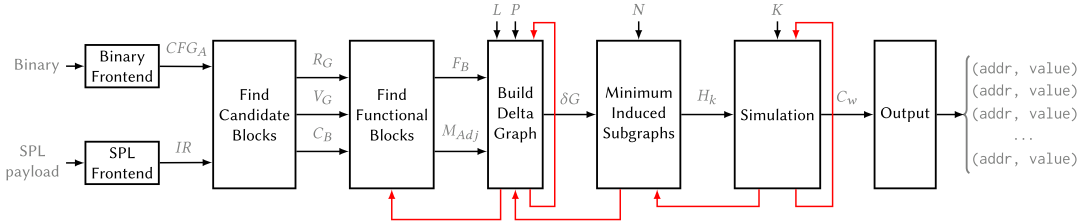
\includegraphics[width=\linewidth]{bopc.png} %
    \caption{\footnotesize{bopc's arch.  The red arrows indicate the iterative process upon failure. CFGA: CFG with basic block abstractions added, IR:Compiled SPL payload RG:Register mapping graph, VG:All variable mapping graphs, CB: Set of candidate blocks, FB: Set of functional blocks, MAdj:Adjacency matrix of SPL payload, $\delta$G:Delta graph, Hk:Induced subgraph, Cw:Constraint set. L:Maximum length of continuous dispatcher blocks, P:Upper bound on payload “shuffles”, N:Upper bound on minimum induced subgraphs, K:Upper bound on shortest paths for dispathers.}}
    \label{fig:bopc}
\end{figure}
\subsection{Results/Evaluation}
They execute 13 SPL payloads applied to 10 popular applications.  BOPC successfully finds payloads and complex execution traces – which would likely not have been found through manual analysis – while following the target’s Control-Flow Graph under an ideal CFI policy in 81\% of the cases. Available at \url{https://github.com/HexHive/BOPC}.

\subsection{Limitations/Comments}
BOPC is limited by the granularity of basic blocks. That is, a combination of basic blocks could potentially lead to the execution of a desired SPL statement, while individual blocks might not. Take for instance an instruction that sets a virtual register to 1. Assume that a basic block initializes rcx to 0, while the following block increments it by 1; a pattern commonly encountered in loops. Al- though there is no functional block that directly sets rcx to 1, the combination of the previous two has the desired eff ect. BOPC can be expanded to address this issue if the basic blocks are coalesced into larger blocks that result in a new CFG.

BOPC sets several upper bounds defined by user inputs. These configurable bounds include the upper limit of (i) SPL payload permutations (P), (ii) length of continuous blocks (L), (iii) of minimum induced subgraphs extracted from the delta graph (N ), and (iv) dispatcher paths between a pair of functional blocks (K). These upper bounds along with the timeout for symbolic execution, reduce the search space, but prune some potentially valid solutions. The evaluation of higher limits may result in alternate or more solutions being found by BOPC.
\newpage
\section{Automatic Heap Layout Manipulation for Exploitation @Security'18}
\subsection{Background/Problems}
As of 2018, the most common approach to solving heap layout manipulation (HLM) problems is manual work by experts.  An analyst examines the allocator’s implementation to gain an understanding of its internals; then, at run-time, they inspect the state of its various data structures to determine what interactions are necessary in order to manipulate the heap into the required layout. The process is complicated by the fact that – when constructing an exploit – one cannot directly interact with the allocator, but instead must use the API exposed by the target program. 

There are four variants of the HLM problem, depending on whether the allocator is deterministic or non-deterministic and whether the starting state is known or unknown. In this paper the authors consider a known starting state and a deterministic allocator, and assume there are no other actors interacting with the heap. 

Their objective in this variant of the HLM problem is as follows: \emph{Given the API for a target program and a means by which to allocate a source and destination buffer, find a sequence of API calls that position the destination and source at a specific offset from each other}.
\subsection{Methods/Techniques}
The authors present the first automatic approach to the problem, based on pseudo-random black-box search. Our approach searches for the inputs required to place the source of a heap-based buffer overflow or underflow next to heap-allocated objects that an exploit developer, or automatic exploit generation system, wishes to read or corrupt. They present a framework for benchmarking heap layout manipulation algorithms, and use it to evaluate our approach on several real-world allocators, showing that pseudo-random black box search can be highly effective. They then present SHRIKE (Fig.\ref{fig:shrike}), a novel system that can perform automatic heap layout manipulation on the PHP interpreter and can be used in the construction of control-flow hijacking exploits. Starting from PHP’s regression tests, SHRIKE discovers fragments of PHP code that interact with the interpreter’s heap in useful ways, such as making allocations and deallocations of particular sizes, or allocating objects containing sensitive data, such as pointers. SHRIKE then uses our search algorithm to piece together these fragments into programs, searching for one that achieves a desired heap layout. SHRIKE allows an exploit developer to focus on the higher level concepts in an exploit, and to defer the resolution of heap layout constraints to SHRIKE. Available at \url{https://sean.heelan.io/heaplayout}.
\begin{figure}[h]
    \centering
    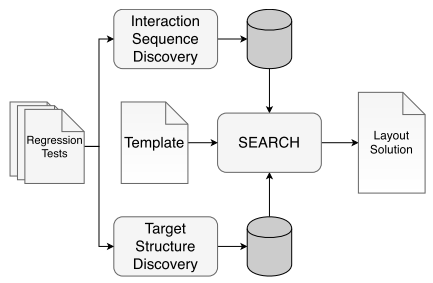
\includegraphics[width=0.7\linewidth]{shrike.png} %
    \caption{shrike's arch.}	
    \label{fig:shrike}
\end{figure}
\subsection{Results/Evaluation}
 They chose the tcmalloc (v2.6.1), dlmalloc (v2.8.6) and avrlibc (v2.0) allocators for experimentation.  They demonstrate this by using SHRIKE in the construction of a control-flow hijacking exploit for the PHP interpreter.  SHRIKE had a 70\% success rate overall, and a 100\% success rate in cases where there was no noise.
\subsection{Limitations/Comments}
Other three variants of the HLM problem are harder than the one addressed in this paper. Some allocators, e.g., Windows system allocator, jemalloc and the DIEHARD family of allocators, do utilise non-determinism to make exploitation more difficult.

Read other references, e.g., [7, 15, 26, 32, 33], for more future works.
\newpage
\section{MarkUs: Drop-in use-after-free prevention for
low-level languages @S\&P'20}

\subsection{Background/Problems}
A variety of techniques have been proposed to mitigate use-after-free vulnerabilities in C and C++. For example, all pointer locations can be logged and then nullified when their data is freed [1], [4], [5], objects allocated with their own page-table entries [6], [7], or probabilistic reuse delays employed [8]–[10]. However, these tend to exhibit both high average- and worst-case overheads in terms of performance and memory utilisation, or have limited coverage.
\subsection{Methods/Techniques}
The authors present MarkUs, a memory allocator that prevents this form of attack at low overhead, sufficient for deployment in real software, even under allocation- and memory-intensive scenarios. MarkUs prevent use-after-free attacks by \emph{quarantining data freed by the programmer and forbidding its reallocation until there are no dangling pointers targeting it}. To identify these MarkUs traverses live-objects accessible from registers and memory, marking those it encounters, to check whether quarantined data is accessible from any currently allocated location. 

Unlike garbage collection, which is unsafe in C and C++, MarkUs ensures safety by \emph{only freeing data that is both quarantined by the programmer and has no identifiable dangling pointers}. The information provided by the programmer’s allocations and frees further allows to optimise the process by freeing physical addresses early for large objects, specialising analysis for small objects, and only performing marking when sufficient data is in quarantine. 
\subsection{Results/Evaluation}
Using MarkUs, they reduce the overheads of temporal safety in low-level languages to 1.1$\times$ on average for SPEC CPU2006, with a maximum slowdown of only 2$\times$, vastly improving upon four state-of-the-art techniques, i.e., Oscar, DangSan, pSweeper and CRCount.
\subsection{Limitations/Comments}
MarkUs fails to detect complex use-after-free vulnerabilities involving hidden pointers, as is a limitation with any technique that involves identifying pointers.

Tagged memory techniques [36,37] can make MarkUs more efficient, by allowing reuse of memory multiple times, based on incrementing the ID tag of each successive allocation, before address space must be quarantined to ensure old IDs have been eliminated and can be reallocated.
\newpage
\section{KARONTE: Detecting Insecure Multi-binary Interactions in Embedded Firmware @S\&P'20}
\subsection{Background/Problems}
Low-power, single-purpose embedded devices (e.g., routers and IoT devices) have become ubiquitous. While they automate and simplify many aspects of users’ lives, recent large-scale attacks have shown that their sheer number poses a severe threat to the Internet infrastructure. Unfortunately, the software on these systems is hardware-dependent, and typically executes in unique, minimal environments with non-standard configurations, making security analysis particularly challenging.  

Many of the existing devices implement their functionality through the use of multiple binaries. This multi-binary service implementation renders current static and dynamic analysis techniques either ineffective or inefficient, as they are unable to identify and adequately model the communication between the various executables.
\subsection{Methods/Techniques}
Based on the intuition that binaries communicate using a finite set of Inter-Process Communication (IPC) paradigms, the authors present KARONTE, a static analysis approach capable of analyzing embedded-device firmware by modeling and tracking multi-binary interactions.  The approach propagates taint information between binaries to detect insecure interactions and identify vulnerabilities.
\begin{figure}[h]
    \centering
    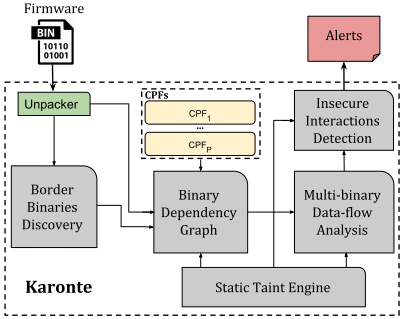
\includegraphics[width=0.7\linewidth]{karonte.png} %
    \caption{karonte's arch.  After unpacking a firmware sample, KARONTE extracts the binaries handling user requests, identifies their data dependencies to build the Binary Dependency Graph (BDG), and uses its inter-binary taint analysis engine to find insecure data flows. CPF: Communication Paradigm Finder.}	
    \label{fig:karonte}
\end{figure}
\subsection{Results/Evaluation}
First, they evaluated KARONTE on 53 firmware samples from various vendors, showing that the tool can successfully track and constrain multi-binary interactions. This led to the discovery of 46 zero-day bugs. Then, they performed a large-scale experiment on 899 different samples, showing that KARONTE scales well with firmware samples of different size and complexity. Available at: \url{https://github.com/ucsb-seclab/karonte}.
\subsection{Limitations/Comments}
KARONTE suffers from the path explosion problem. 
they limit path explosion by: (i) providing precise taint propagation policies, (ii) using timeouts, (iii) limiting loop iterations, and (iv) automatically creating function summaries.

Karonte may generate both false positives and false negatives. They are due to the fact that taint information might not be correctly propagated to unfollowed paths (e.g., due to time, call-stack depth, or loop constraints), or imprecisions of the underlying static analysis tool (i.e., angr). This might result in incomplete BDGs, and, therefore, some security vulnerabilities might be left undiscovered. 

Though by default, KARONTE finds buffer overflows and denial-of-service vulnerabilities, its design allows an analyst to support different types of vulnerabilities. For instance, an analyst can extend Karonte to find use-after-free bugs by providing a new detection module, such as [16].
\newpage
\section{What You Corrupt Is Not What You Crash: Challenges in Fuzzing Embedded Devices @NDSS'18}
\subsection{Background/Problems}
While common desktop systems have a variety of mechanisms to detect faulty states (e.g., segmentation faults, heap hardening and sanitizers) and to analyze them (e.g., command-line return values or core dumps), embedded devices often lack such mechanisms because of their limited I/O capabilities, constrained cost, and limited computing power.  As a result, \emph{silent memory corruptions} occur more frequently on embedded devices than on traditional computer systems, creating a significant challenge for conducting fuzzing sessions on embedded systems software.
\subsection{Methods/Techniques}
The authors analyze the challenges of fuzzing embedded devices (fault detection, performance and scalability, instrumentation), make a classification of embedded systems with respect to the difficulty of detecting memory corruptions in their software, evaluate the real world effects of different memory corruptions on those classes of embedded systems, describe the techniques that can be used for improving fuzzing on embedded devices, and present six heuristics that can be used to detect faults due to the memory corruption (tracking segment, format specifier, heap object, stack object, call stack, call frame, respectively, Fig.\ref{fig:liveanalysis}), when the firmware of an embedded system can be run in either a partial or full emulation environment.
\begin{figure}[h]
    \centering
    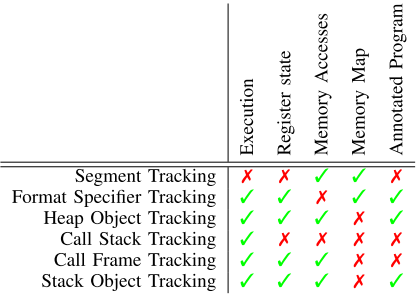
\includegraphics[width=0.6\linewidth]{liveanalysis.png} %
    \caption{Deployed live analysis techniques and their requirements.}	
    \label{fig:liveanalysis}
\end{figure}
\subsection{Results/Evaluation}
They implemented the heuristics on top of a combination of the Avatar [54] and PANDA [13] frameworks. They use PANDA to emulate the firmware and rely on its plugin system to obtain live feedback over the execution of a partial or fully emulated firmware. Avatar allows the tester to save and replay the device state after it is initialized. 

They conducted a number of tests to show their effectiveness and their overhead in a fuzzing experiment. Experiments show that partial emulation significantly reduces the fuzzing throughput. However, when full emulation is possible, this setup can combine the best of both worlds and detect 100\% of the corrupting inputs while improving the fuzzing efficiency beyond what could be obtained using the physical device. Available at: \url{https://github.com/avatartwo/ndss18_wycinwyc}.
\subsection{Limitations/Comments}
They relied on artificial bugs in the experiments, which lacks of evidents in real applications. When migrating from an artificial test scenario to real world software, the observed false positive and negative rates of the individual heuristics will vary.

The ability to fully emulate arbitrary firmware images is still an open problem. Therefore, the solution discussed in this paper may not be applicable to all scenarios and all embedded devices. 

\newpage

\section{Looking from the Mirror: Evaluating IoT Device Security through Mobile Companion Apps @Security'19}
\subsection{Background/Problems}
Smart home IoT devices have increasingly become a favorite target for the cybercriminals due to their weak security designs. To identify these vulnerable devices, existing approaches rely on the analysis of either real devices or their firmware images. These approaches, unfortunately, are difficult to scale in the highly fragmented IoT market due to the unavailability of firmware images and the high cost involved in acquiring real-world devices for security analysis.

\subsection{Methods/Techniques}
The authors present a platform (Fig.\ref{fig:mirror}) that accelerates vulnerable device discovery and analysis, without requiring the presence of actual devices or firmware. Our approach is based on two key observations: First, IoT devices tend to reuse and customize others’ components (e.g., software, hardware, protocol, and services), so vulnerabilities found in one device are often present in others. Second, reused components can be indirectly inferred from the mobile companion apps of the devices; so a cross analysis of mobile companion apps may allow us to approximate the similarity between devices.

(1) app analysis: find the characteristics of a device by analyzing its companion app, and (2) cross-app analysis: find device families, i.e. cluster of devices, that have similarity in some of the characteristics found in app analysis by analyzing multiple apps. Clustering helps identify apps that have a similar set of vulnerabilities based on shared components.
\begin{figure}[h]
    \centering
    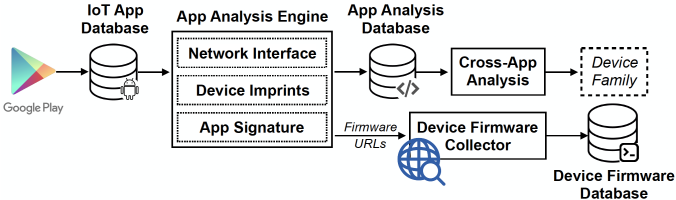
\includegraphics[width=\linewidth]{mirror.png} %
    \caption{mirror's arch.}	
    \label{fig:mirror}
\end{figure}
\subsection{Results/Evaluation}
They perform a large-scale analysis involving over 4,700 devices and  2000 apps. Their study brings to light the sharing of vulnerable components across the smart home IoT devices (e.g., shared vulnerable protocol, backend services, device rebranding), and leads to the discovery of 324 devices from 73 different vendors that are likely to be vulnerable to a set of security issues.

\subsection{Limitations/Comments}
The major limitation of the approach is the accuracy of the analysis results. As the analysis solely on mobile companion apps, the information obtained may not be an accurate reflection of the device. For example, a device may have patched a vulnerability and the patch did not change the device interfaces at all. In this case, the analysis will still output the device as potentially vulnerable. A multi-stage solution can help address this limitation where the first stage (i.e., the platform) narrows down the scope of analysis by identifying the potentially vulnerable devices, and the second stage automates the vulnerability confirmation with more targeted but rigorous analysis, e.g., dynamic/static analysis of firmware, device fuzzing.

Another limitation of the approach is that the network interface analysis can be rendered less effective in scenarios where IoT backend servers or cloud significantly decouple device interfaces from app interfaces. An example is the Google and Amazon devices where much of the management is done through the cloud.

Another aspect to improve on is the dimension and granularity of the similarity analysis. Further improvements to the App Analysis Engine may allow the platform to detect similarities in finer components of a device software stack (e.g., web server, PHP interpreter, web application, OS, driver) as well as other dimensions (e.g., similar developer, similar development toolchain). This would enable us to track vulnerability propagation more comprehensively and accurately. 
\newpage
\section{PeriScope: An Effective Probing and Fuzzing Framework for the Hardware-OS Boundary @NDSS'19}
\subsection{Background/Problems}
Currently, most of the kernel’s attack surface is situated along the system call boundary. Ongoing kernel protection efforts have focused primarily on securing this boundary.  However, there are additional paths to kernel compromise that do not involve system calls, as demonstrated by several recent exploits. For example, by compromising the firmware of a peripheral device such as a Wi-Fi chipset and subsequently sending malicious inputs from the Wi-Fi chipset to the Wi-Fi driver, adversaries have been able to gain control over the kernel without invoking a single system call. Unfortunately, there are currently no practical probing and fuzzing frameworks that can help developers find and fix such vulnerabilities occurring along the hardware-OS boundary.
\subsection{Methods/Techniques}
The authors present PERISCOPE (Fig.\ref{fig:periscope}), a Linux kernel based probing framework that enables fine-grained analysis of device-driver interactions. PERISCOPE hooks into the kernel’s \emph{page fault handling} mechanism to either passively monitor and log traffic between device drivers and their corresponding hardware, or mutate the data stream on-the-fly using a fuzzing component, PERIFUZZ, thus mimicking an active adversarial attack. PERIFUZZ accurately models the capabilities of an attacker on peripheral devices, to expose different classes of bugs including, but not limited to, memory corruption bugs and double-fetch bugs. 
\begin{figure}[h]
    \centering
    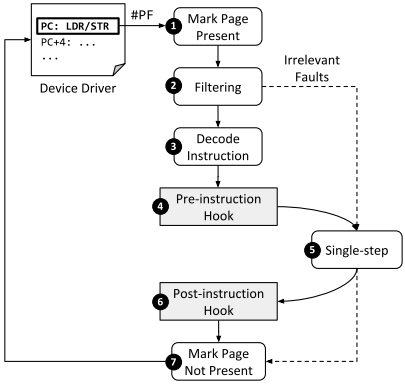
\includegraphics[width=0.7\linewidth]{periscope.png} %
    \caption{periscope's arch.}	
    \label{fig:periscope}
\end{figure}
\subsection{Results/Evaluation}
To demonstrate the risk that peripheral devices pose, as well as the value of their framework, they have evaluated PERIFUZZ on the Wi-Fi drivers of two popular chipset vendors\footnote{The Google Pixel 2 and Samsung Galaxy S6 are equipped with Qualcomm and Broadcom chipsets, respectively.}, where they discovered 15 unique vulnerabilities, 9 of which were previously unknown. Available at: \url{https://github.com/securesystemslab/periscope}.
\subsection{Limitations/Comments}
\emph{Augmenting the fuzzing engine:} Like DIFUZE [35], static analysis can be introduced to infer the type of an I/O buffer, which can save fuzzing cycles by respecting the target type when mutating a value. The dependencies between device-driver interaction messages can also be inferred using static and trace analysis techniques [41], [58], which can help fuzzing stateful device-driver interaction protocols. Alternatively, developers can specify the format of an I/O buffer and/or interaction protocol in a domain-specific language [10], [75]. In addition to improving the mutation of the data stream, they could use system call fuzzers such as Syzkaller that generate different user-space programs [75].  These generated programs could actively send requests to the driver and potentially to the device, which in turn can increase reachable interrupt code paths.

\emph{Combining with Dynamic Analysis:}
PeriScope runs in a concrete execution environment; thus, existing dynamic analysis tools can be used to uncover silent bugs. For example, kernel sanitizers such as address sanitizer and undefined behavior sanitizer can complement their fuzzer [48], [63]. Memory safety bugs often silently corrupt memory without crashing the kernel. PeriFuzz, by itself, cannot reveal such bugs. When combined with a sanitizer, however, these bugs would be detected. Other dynamic analysis techniques such as dynamic taint tracking can also be adapted to detect security-critical semantic bugs such as passing security-sensitive values (e.g., kernel virtual addresses) to untrusted peripherals.

Crashes in kernel space cause a system reboot, which significantly lowers the throughput of any kernel fuzzer.  They circumvented this problem by disabling certain code paths that contain previously discovered shallow bugs. However, this does reduce the effectiveness of PeriFuzz as it cannot traverse the subpaths rooted at these blacklisted bugs. Note that this problem also affects other kernel fuzzers, e.g., DIFUZE and Syzkaller.

Due to the significant latency involved in system restarts, whole-system fuzzers typically fuzz the system without restarting it between fuzzing iterations.  This can limit the effectiveness of such fuzzers, because the internal states of the target system persist across iterations.  Changing internal states can also lead to instability in the coverage-guidance, as the same input can exercise different code paths depending on the system state. This means that coverage-guidance may not be fully effective.  Existing device driver checkpointing and recovery mechanisms could be adapted to alleviate the problem [46], [70], because they provide mechanisms to roll drivers back to an earlier state. Such a roll back takes significantly less time than a full system reboot.
\newpage

\section{PARTEMU: Enabling Dynamic Analysis of Real-World TrustZone Software Using Emulation @Security'20}
\subsection{Background/Problems}
ARM’s TrustZone technology is the basis for security of billions of devices worldwide, including Android smartphones and IoT devices. Because TrustZone has access to sensitive information such as cryptographic keys, access to TrustZone has been locked down on real-world devices: only code that is authenticated by a trusted party can run in TrustZone. A side-effect is that TrustZone software cannot be instrumented or monitored. Thus, recent advances in dynamic analysis techniques such as feedback-driven fuzz testing have not been applied to TrustZone software. Researchers have been restricted to primarily static reverse-engineering of binaries to find vulnerabilities in TrustZone software.
\subsection{Methods/Techniques}
The authors build an emulator that runs four widely-used, real-world TrustZone operating systems (TZOSes) - Qualcomm’s QSEE, Trustonic’s Kinibi, Samsung’s TEEGRIS, and Linaro’s OP-TEE - and the trusted applications (TAs) that run on them. The traditional challenge for this approach is that the emulation effort required is often impractical. However, they find that TZOSes depend only on a limited subset of hardware and software components. By carefully choosing a subset of components to emulate (Fig.\ref{fig:partemu}), they make the effort practical and implement the emulation on PARTEMU, a modular framework they develop on QEMU and PANDA.
\begin{figure}[h]
    \centering
    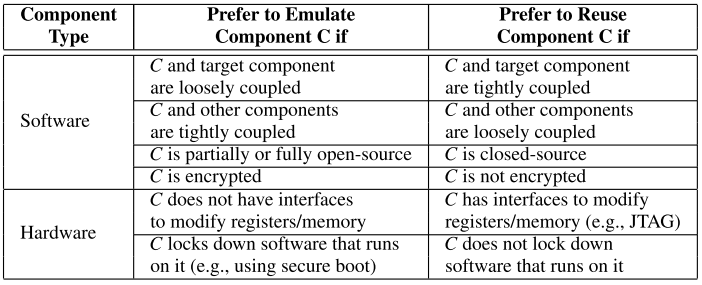
\includegraphics[width=.9\linewidth]{partemu.png} %
    \caption{Criteria to decide whether to reuse or emulate a component C. As in object-oriented design, they use “loosely-coupled” to mean components that have well-defined interfaces with each other and work largely independently of each other, and “tightly-coupled” to mean the opposite, that is, components that need to know each others’ internal data structure implementations, leading to complicated interfaces and deep dependencies.}	
    \label{fig:partemu}
\end{figure}
\subsection{Results/Evaluation}
They show the utility of PARTEMU by integrating feedback-driven fuzz-testing using AFL and use it to perform a large-scale study of 194 unique TAs from 12 different Android smartphone vendors and a leading IoT vendor, finding previously unknown vulnerabilities in 48 TAs, several of which are exploitable. They identify patterns of developer mistakes unique to TrustZone development that cause some of these vulnerabilities, highlighting the need for TrustZone-specific developer education.  They also demonstrate using PARTEMU to test the QSEE TZOS itself, finding crashes in code paths that would not normally be exercised on a real device. Our work shows that dynamic analysis of real-world TrustZone software through emulation is both feasible and beneficial.
\subsection{Limitations/Comments}
Dealing with Stateful TAs. On a random sample of 10 TAs, AFL had basic-block coverage varying from 0.2\% to 45.6\% with a median of 17.7\%. A major limiting factor for coverage was TA state: they noticed that several TAs had internal finite state machines and therefore required a sequence of multiple inputs to drive them to interesting states (e.g., connected, authorized, processing). Our driver currently sends a single message to a newly forked TA instance each time so that AFL does not have issues with stability. Therefore, they cannot get past state checks, which require a sequence of inputs.

Hardware Roots of Trust. PARTEMU does not emulate hardware roots of trust. An example is the factory-installed per-device private key signed by the Samsung CA and used for remote attestation. Thus, code paths in TAs that depend on remote attestation succeeding may not work. For example, Samsung Pay uses remote attestation for credit card enrollment; they cannot successfully enroll a credit card using a Samsung Pay TA running on PARTEMU because they do not have access to the attestation key that would be present on a real device.

Performance. Since they ran PARTEMU on an x86 machine, they could not take advantage of ARMv8 hardware virtualization. AFL ran at around 10-25 executions per second for QSEE, OP-TEE, and TEEGRIS, while their performance optimizations for Kinibi enabled 125 executions per second. Thus, a future work is to explore running PARTEMU directly on ARMv8 hardware.
\newpage

\section{Enhancing example-based code search with functional semantics @The Journal of Systems and Software'20}
\subsection{Background/Problems}
As the quality and quantity of open source code increase, effective and efficient search for code implementing certain semantics, or semantics-based code search, has become an emerging need for software developers to retrieve and reuse existing source code. Previous techniques in semantics-based code search encode the semantics of loop-free Java code snippets as constraints and utilize an SMT solver to find encoded snippets that match an input/output (IO) query.
\subsection{Methods/Techniques}
The authors present in this article the Quebio approach to semantics-based search for Java methods. Quebio advances the state-of-the-art by supporting important language features like invocation to library APIs and enabling the search to handle more data types like array/List, Set, and Map. Compared with existing approaches, Quebio also integrates a customized keyword-based search that uses as the input a textual, behavioral summary of the desired methods to quickly prune the methods to be checked against the IO examples.
\begin{figure}[h]
    \centering
    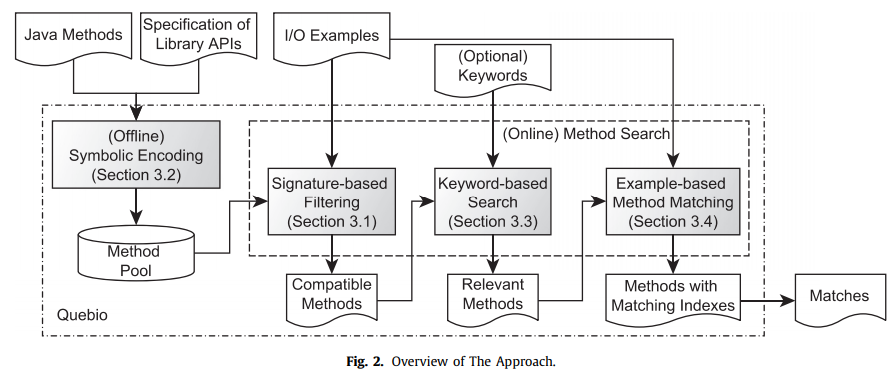
\includegraphics[width=.9\linewidth]{codesearch_semantic_based.png} %
    \caption{semantics-based search for Java method using IO examples}	
    \label{fig:codesearch_semantic_based}
\end{figure}
\subsection{Results/Evaluation}
conducted experiments on 47 queries based on real-world questions from programmers to evaluate our approach. The approach was able to find correct methods from a pool of 14,792 candidates for 43 of the queries, spending on average 213.2 seconds on each query. Such results suggest our approach is both effective and efficient.
\subsection{Limitations/Comments}
A threat to external validity concerns the limited data types that Quebio supports in its current implementation.While Quebio has the ability to handle API calls in candidate methods, the availability and the complexity of logical formulas encoding those APIs’ semantics can present challenges to Quebio in achieving similar levels of effectiveness and efficiency on other queries. In the future, we plan to extend Quebio to support more data types.
\newpage

\section{Active Inductive Logic Programming for Code Search @ICSE'20}
\subsection{Background/Problems}
Modern search techniques either cannot efficiently incorporate human feedback to refine search results or cannot express structural or semantic properties of desired code.
\subsection{Methods/Techniques}
The authors present in this article the Quebio approach to semantics-based search for Java methods. Quebio advances the state-of-the-art by supporting important language features like invocation to library APIs and enabling the search to handle more data types like array/List, Set, and Map. Compared with existing approaches, Quebio also integrates a customized keyword-based search that uses as the input a textual, behavioral summary of the desired methods to quickly prune the methods to be checked against the IO examples.

\subsection{Results/Evaluation}
On average, ALICE successfully identifies similar code locations with 93\% precision and 96\% recall in 2.7 search iterations. ALICE achieves 100\% precision and 97\% recall in the first dataset, while it achieves 75\% precision and 94\% recall in the second dataset. The reason is that the second dataset contains code fragments that loop over a double array with no write to output operations, which is a semantic constraint imposed by Casper [20] for loop optimization. However, ALICE does not learn predicates that differentiate read and write operations on an array and therefore returns a large number of code fragments that write double arrays in a loop, which leads to low precision.
compare with critics:
In six out of seven cases, ALICE achieves the same or better precision and recall with fewer iterations to converge, compared to Critics. In ID 4, ALICE has low precision because the expected code contains a switch statement, which is currently not extracted by ALICE as a logic fact. Extending current logic predicates to support more syntactic constructs remain as future work.
\subsection{Limitations/Comments}
we generate facts based on structural and intra-procedural control flow properties. Other types of analysis such as dataflow analysis or aliasing analysis could be used in identifying similar snippets. In addition, the query language itself can be extended to make it easier to capture the properties of desired code. For example, by introducing negations in the query language,a user can specify atoms that should not be included. There could be specializations that strictly require negations. However, in our experiments, empirically, we are always able to find a pattern without negations. As mentioned in Section III-D, our learning process is monotonic and to learn a different query, a user may need to start over. To overcome this, we may need backtracking and investigate new search algorithms that generalize and specialize the query in a different way.
\newpage

\section{LTRWES:A new framework for security bug report detection @Information and Software Technology'20}
\subsection{Background/Problems}
it is important to identify SBRs quickly and accurately among bug reports (BRs) that have been disclosed in bug tracking systems.Although a few methods have been already proposed for the detection of SBRs, challenging issues still remain due to noisy samples, class imbalance and data scarcity.
\subsection{Methods/Techniques}
LTRWES is a content-based data filtering and representation framework that has several desirable properties not shared in other methods. 
Firstly, it exploits ranking model to efficiently filter non-security bug reports (NSBRs) that have higher content similarity with respect to SBRs. 			
Secondly, it applies word embedding technology to transform the rest of NSBRs, together with SBRs, into low-dimensional real-value vectors
\begin{figure}[h]
    \centering
    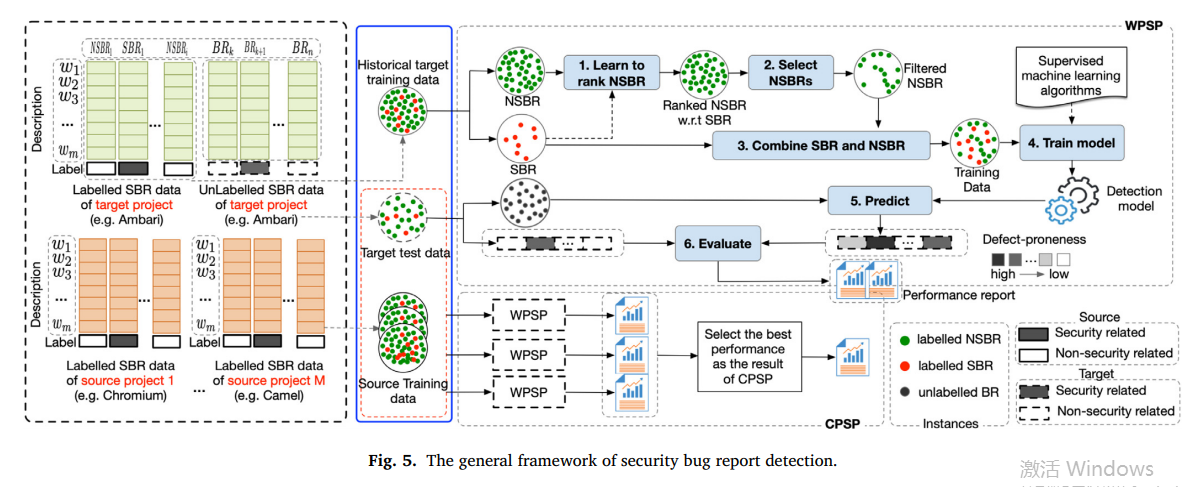
\includegraphics[width=.9\linewidth]{security_bug_report_detection.png} %
    \caption{the general framework of security bug report detection}	
    \label{fig:security_bug_report_detection}
\end{figure}
\subsection{Results/Evaluation}
The highest g-measure for each project is obtained by LTRWES. LTRWES outperforms FARSEC on average by 16.7\% and 22.4\% in gmeasure for WPSP and CPSP respectively
LTRWES outperforms FARSEC by 25.4\% and 54.5\% on average in recall for WPSP and CPSP.
\subsection{Limitations/Comments}
Our future work includes: 1) develop an improved method that use more projects as sources to further improve the performance of crossproject SBRs prediction, 2) combine textual information with side information in bug reports (such as product, component) to improve the performance of SBRs prediction, 3) develop more effective methods to reduce the false positive rate while maintaining high true positive rate in detecting security bug reports, and 4) adopt other hyperparameter tuning methods to further improve the performance of prediction models.
\newpage

\section{Search-Based Test and Improvement of Machine-Learning-Based Anomaly Detection Systems @ISSTA'19}
\subsection{Background/Problems}
the live learning mechanism,progressively injecting small portions of abnormal data. swift the learned states to a point where harmful data can pass unnoticed.
\subsection{Methods/Techniques}
\begin{itemize}
	\item \textbf{Search-Based Test of IDS(intrusion detection systems):}
          --Genotype;
          --Fitness function;(the distance between target and the closest cluster centroid and minimizing the consumed time budget)
         --Selectors ( keeps the best individuals out of samples of three)
         --alterers(single-point crossover with a 0.2 recombination probability, while gene mutation in the offspring occurs with a probability of 0.15)
    \item \textbf{Search-Based Improvement of IDS:}
          --Genotype;
          --Fitness function(fastest detection time, minimizing resources);
          --Selectors and alterers
	\item \textbf{Co-Evolution of Attacks and Defences:}	  
\end{itemize}

\subsection{Results/Evaluation}
\textbf{dataset:}4SICS Geek Lounge dataset, contains 18 hours of real SCADA
traffic data. detecting DoS training attacks over a network
\textbf{results:}The defences resulting from the highest iterations detected 49 attacks out of 50.
\subsection{Limitations/Comments}
\begin{itemize}
	\item We design a testing framework based on search algorithms that, given an IDS, can generate a test (i.e. a training attack scheme) to deceive the IDS. We instantiate this framework in a denial-of-service attack scenario, where a training attack consists of unnoticed, successive increases in data rate. 
	\item We generalize the countermeasure proposed by Muller et al. [11] and design a genetic algorithm to search for a defence strategy (in the form of new parameter sets) that succeeds in detecting the attack induced by a given test case.
	\item We show that our testing framework enables the continuous improvement of IDS detection capabilities. More precisely, we set up a co-evolution process that attractively generates attacks and defences leading to new parameter sets that make the IDS resilient to all generated attacks.
\end{itemize}
\newpage

\section{Codebase-adaptive detection of security-relevant methods @ISSTA'19}
\subsection{Background/Problems}
users must configure the static tools with lists of security-relevant methods (Srm) that are relevant to their development context.aids analysis users in detecting Srm.
\subsection{Methods/Techniques}
\begin{itemize}
	\item \textbf{Features:}uses a set of binary features that evaluate certain properties of the methods,constructs a feature matrix ; identified 25 feature types, instantiated as 206 concrete features,\textbf{Classifiers:}Support Vector Machine (SVM), Bayes Net, Naive Bayes, Logistic
Regression, C4.5, Decision Stump, and Ripper
    \item  take user feedback into account, allowing developers to adapt SWAN to the code base
\end{itemize}

\subsection{Results/Evaluation}
\textbf{datsets:}twelve popular Java frameworks
\textbf{results:}SWAN achieves an average precision of 0.826, which is better or comparable to existing approaches.SWANAssist requires a relatively low effort from the developer to significantly improve its precision.

\subsection{Limitations/Comments}
It is possible to improve the precision of static analyses by providing more granular Srm information. Not only the methods themselves are important, which objects they affect can also be important
(i.e., which parameter, static variable, return variable, or base object).Additionally, we plan to extend SWAN and SWANAssist to support a larger number of CWEs. We also plan to improve SWAN’ training set in a more systematic manner, to ensure a better precision of the approach, and develop a better strategy to handle potentially problematic methods in SuggestSWAN
\newpage
\end{document}
